\jxhj{%教学后记
	}
\skrq{%授课日期
	2017年11月30日 4-5节}
\ktmq{%课题名称
	 Siemens上的孔加工指令}
\jxmb{%教学目标,每行前面要加 \item
	\item 掌握孔加工的加工工艺;
	\item 掌握Siemens上的孔加工指令的选用;
	\item 掌握Siemens上孔加工指令的使用;
	\item 会进行孔加工程序的编写。}
\jxzd{%教学重点,每行前面要加 \item
	\item Siemens上孔加工指令的使用;
	\item 进行孔加工程序的编写。 }
\jxnd{%教学难点,每行前面要加 \item
	\item 进行孔加工程序的编写。 }
\jjff{%教学方法
	通过讲述、举例、演示法来说明;}

\makeshouye %制作教案首页

%%%%教学内容
\subsection{组织教学}
\begin{enumerate}[\hspace{2em}1、]
	\item 集中学生注意力;
	\item 清查学生人数;
	\item 维持课堂纪律;
\end{enumerate}

\subsection{复习导入及主要内容}
\begin{enumerate}[1、]
\item 一行孔的编程;
\item 一列孔的编程;
\item 斜线孔系的编程;
\item 多行孔系的编程。
\end{enumerate}

\subsection{教学内容及过程}
\subsubsection{SIEMENS 孔加工循环概述}
SIEMENS上的固定循环就是一些工艺子程序,分为钻削循环
、钻孔样式循环和铣削循环。

名称如下:

\begin{enumerate}
	\item 钻孔循环 
\begin{itemize}
\item 	CYCLE81    钻孔,中心钻孔 
\item CYCLE82    中心钻孔 
\item CYCLE83    深度钻孔 
\item CYCLE84    刚性攻丝 
\item CYCLE840   带补偿卡盘攻丝 
\item CYCLE85    铰孔1(镗孔1) 
\item CYCLE86    镗孔(镗孔2) 
\item CYCLE87    铰孔2(镗孔3) 
\item CYCLE88    镗孔时可以停止1(镗孔4) 
\item CYCLE89    镗孔时可以停止2(镗孔5)

\end{itemize}
\vspace{10pt}

\item 钻孔样式循环  
\begin{itemize}
	\item HOLES1    加工一排孔 
\item HOLES2    加工一圈孔  
\end{itemize}
\vspace{10pt}
\item 铣削循环 
\begin{itemize}
	\item CYCLE71    端面铣削 
\item CYCLE72    轮廓铣削 
\item CYCLE76    矩形过渡铣削 
\item CYCLE77    圆弧过渡铣削 
\item LONGHOLE   槽 
\item SLOT1    圆上切槽 
\item SLOT2    圆周切槽 
\item POCKET3    矩形凹槽 
\item POCKET4    圆形凹槽 
\item CYCLE90    螺纹铣削
\end{itemize}

\end{enumerate}
\vspace{10pt}
编程器中图形循环支持,根据图形直观的输入参数。

\subsubsection{孔加工固定循环指令}

钻孔,中心孔-CYCLE81

格式:CYCLE81(RTP,RFP,SDIS,DP,DPR)

RTP 后退平面(绝对) 

RFP 参考平面(绝对) 

SDIS 安全间隙(无符号输入) 

DP 最后钻孔深度(绝对) 

DPR相当于参考平面的最后钻孔深度(无符号输入)

\begin{figure}[h]
	\centering
	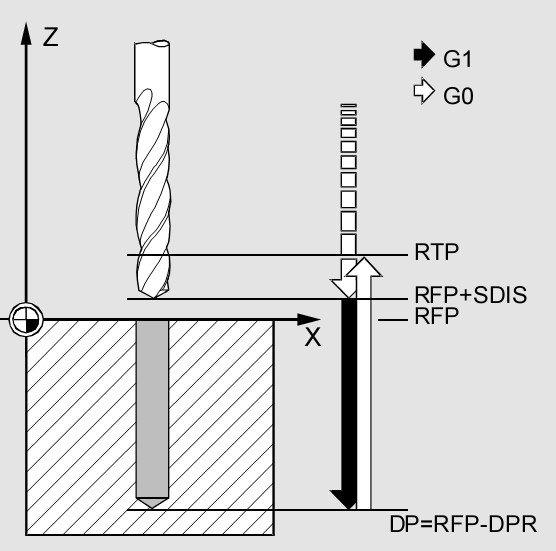
\includegraphics[width=0.7\linewidth]{data/image/23-1}
	\caption{动作顺序}
	\label{fig:23-1}
\end{figure}

如果一个值同时输入给DP和DPR,最后钻孔深度则来自DPR。

CYCLE82(RTP,RFP,SDIS,DP,DPR,DTB)

RTP Real 后退平面(绝对)

RFP Real 参考平面(绝对) 

SDIS Real 安全间隙(无符号输入) 

DP Real 最后钻孔深度(绝对)
 
DPR Real 相当于参考平面的最后钻孔深度(无符号输入) 

DTB Real 最后钻孔深度时的停顿时间(断屑)

\begin{figure}[h]
	\centering
	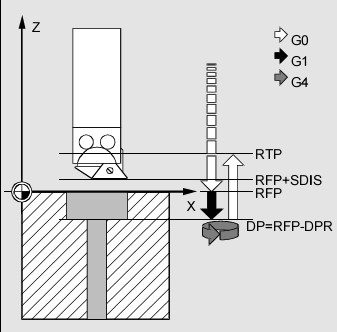
\includegraphics[width=0.7\linewidth]{data/image/23-2}
	\caption{动作顺序}
	\label{fig:23-2}
\end{figure}

CYCLE85(RTP,RFP,SDIS,DP,DPR,DTB,FFR,RFF)

RTP Real 退回平面(绝对值) 

RFP Real 参考平面(绝对值) 

SDIS Real 安全间隙(无符号输入) 

DP Real 最后钻孔深度(绝对值) 

DPR Real 相对于参考平面的最后钻孔深度(无符号输入) 

DTB Real 最后钻孔深度时的停顿时间(断屑) 

FFR Real 进给率 

RFF Real 退回进给率

\begin{figure}[h]
	\centering
	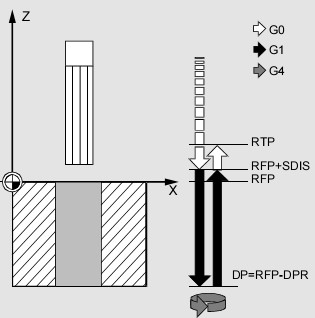
\includegraphics[width=0.7\linewidth]{data/image/23-3}
	\caption{动作顺序}
	\label{fig:23-3}
\end{figure}

注意: 循环调用前设定好率,主轴转速和和转向,
循环调用前必须使刀具到达钻孔位置,
之前的G功能,之后还有效。

\subsubsection{模态调用}

在有MCALL指令的程序段中调用子程序,如果其后的程序段中含有轨迹运行,则子程序会自动调用。该调用一直有效,直到调用下一个程序段。 

用MCALL指令模态调用子程序的程序段以及模态调用结束指令均需要一个独立的程序段。

比如可以使用MCALL指令来方便地加工各种排列形状的孔。

N10 MCALL CYCLE82(…)      ;钻削循环82 

N20 HOLES1(…)    ;行孔循环,在每次到达孔位置之
后,使用传送参数执行CYCLE82(…)循环 

N30 MCALL    ;结束CYCLE82(…)的模态调用

\subsubsection{加工实例}

加工如\ref{fig:21-2}所示的零件,其中孔的有效深度为30mm。

\begin{figure}
	\centering
	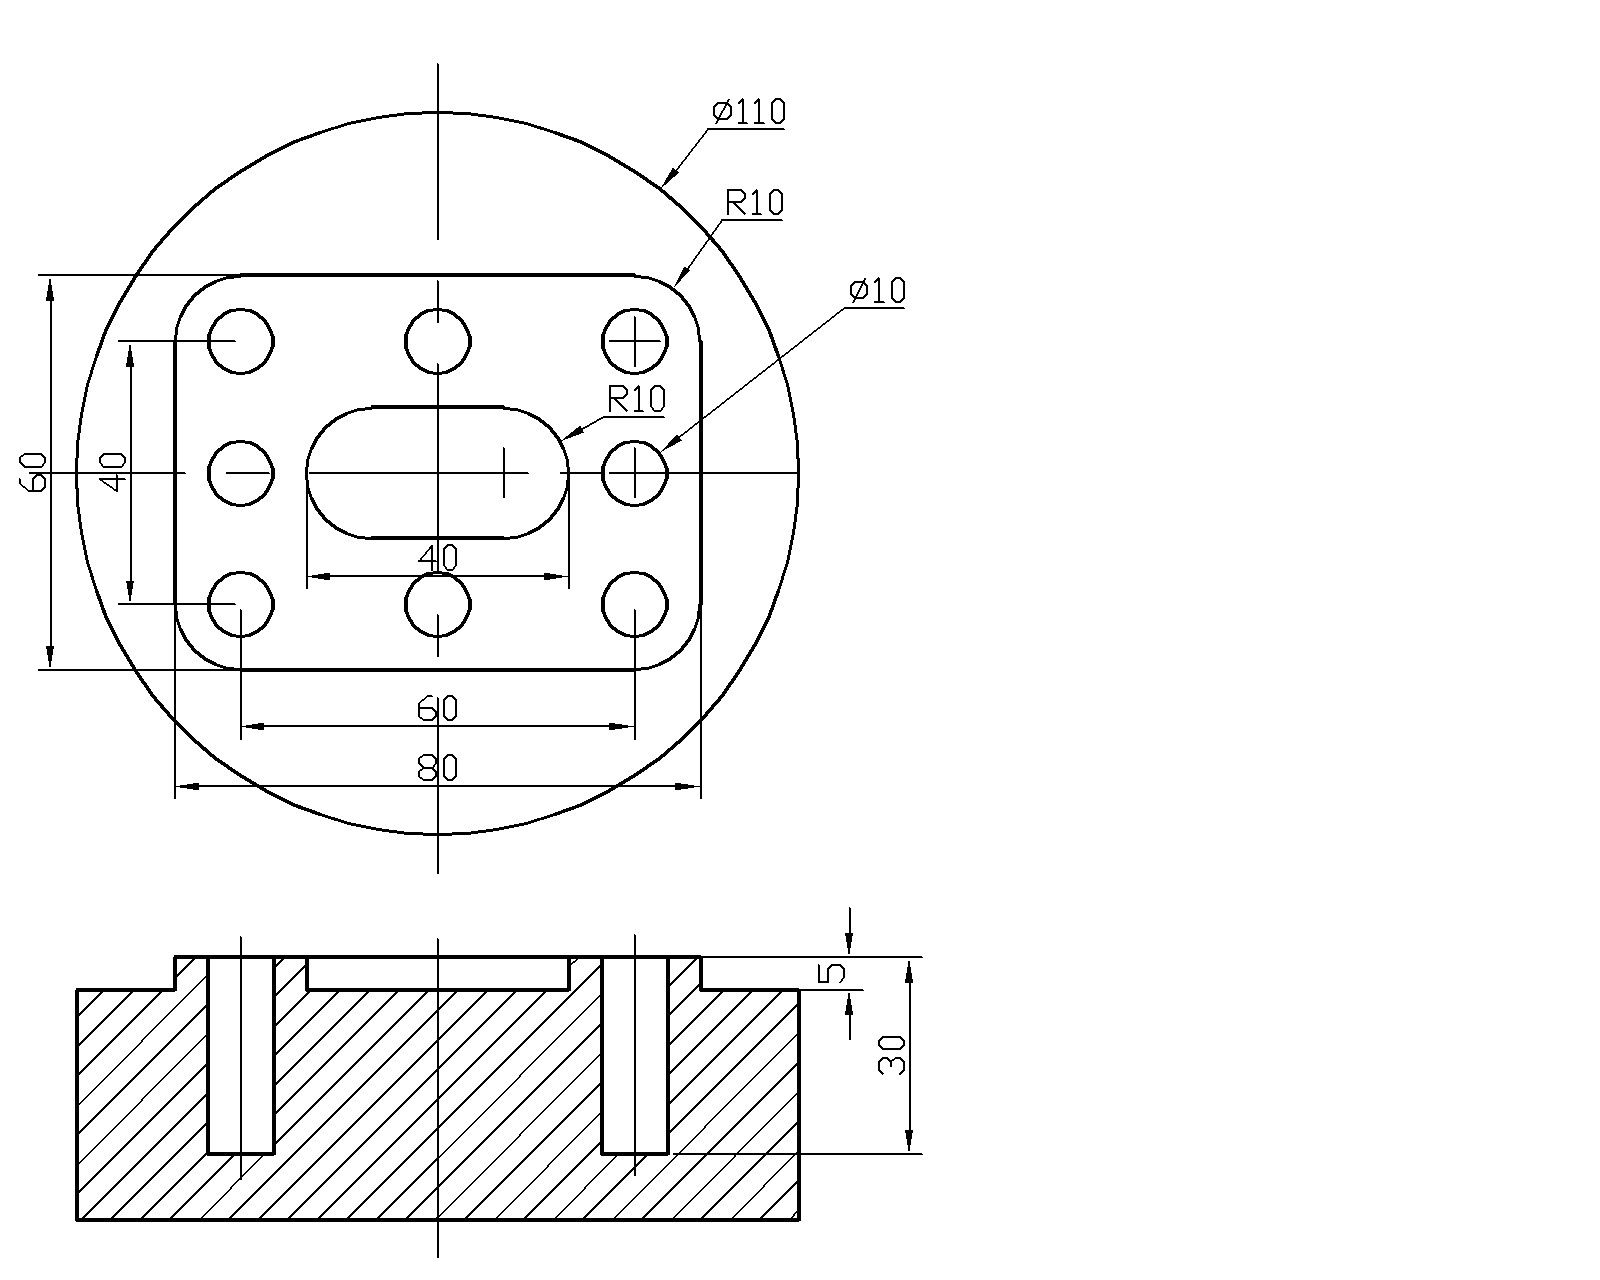
\includegraphics[width=0.5\linewidth,trim=0 0 450  0,clip]{data/image/21-2}
	\caption{孔加工实例}
	\label{fig:21-2}
\end{figure}

1、孔加工方法:钻中心孔、钻孔、铰孔

2、刀具:

$\varnothing $ 3中心钻(切削刃长10mm,加工深度6-8mm,粗对刀即可)S1200 F120 Z-6.0

$\varnothing $ 9.8麻花钻 S550 F80.0 Z-35.0 (比32多3mm)

$\varnothing $ 10机用铰刀 S300 F50 Z-32.0 (比30多2mm)

4、参考程序:
\begin{lstlisting}
GX01
G54G17G40G90
M3S1000
G1Z30.F2000
F60
MCALL CYCLE81(30,0,3,-8,8)
G0X-30Y20
X0
Y20
X30
Y0
Y-20
X0
X-30
Y0
MCALL
M5
M2
\end{lstlisting}



\subsection{课堂小结}
\begin{enumerate}[1、]
\item Siemens孔加工循环概述;
\item 孔加工固定循环指令;
\item 模态调用;
\item 加工实例。
\end{enumerate}

\vfill
\subsection{布置作业}
\begin{enumerate}[1、]
	\item 综合习题一。
\end{enumerate}
\vfill